\section{Classical Mismatch Costs and Diagnostic Limits}\label{sec:zones}
For a centred scalar observation with fixed effective noise variance $q$ and signal variance $p$, the matched Wiener gain is $R=p/(p+q)$. An estimator assuming variance $\kappa p$ uses $g=\kappa R/(1-R+\kappa R)$. The normalised excess error is a classical identity:
\begin{proposition}[Scalar mismatch cost]\label{prop:mismatch}
\begin{equation}\label{eq:delta}
\Delta(R,\kappa)=\frac{R(1-R)^2(\kappa-1)^2}{(1-R+\kappa R)^2}.
\end{equation}
\end{proposition}
The proof in Appendix~\ref{app:proof} separates this identity from its experimental approximations. In absolute units, for true power $P$, assumed power $Q$ and unchanged effective noise $N$,
\begin{equation}\label{eq:delta-abs}
P\Delta=\frac{N^2(Q-P)^2}{(P+N)(Q+N)^2}.
\end{equation}
Under-estimation has limit $\Delta\to R$ as $\kappa\to0$, whereas over-estimation has limit $(1-R)^2/R$ as $\kappa\to\infty$. The latter exceeds signal energy at $R<(3-\sqrt5)/2$; total error exceeds zero reconstruction when $\Delta>R$. Neither statement defines a universal safe bandwidth.
\begin{corollary}[Reciprocal mismatch]\label{cor:flip}
For $0<R<1$ and $\kappa>1$, $\Delta(R,\kappa)>\Delta(R,1/\kappa)$ if and only if $R<1/2$.
\end{corollary}
The effective noise is held fixed, including any aliased components represented by it. Changing several powers in an alias set or using a non-diagonal sampling operator need not preserve this scalar reduction.

\begin{figure*}[t]\centering
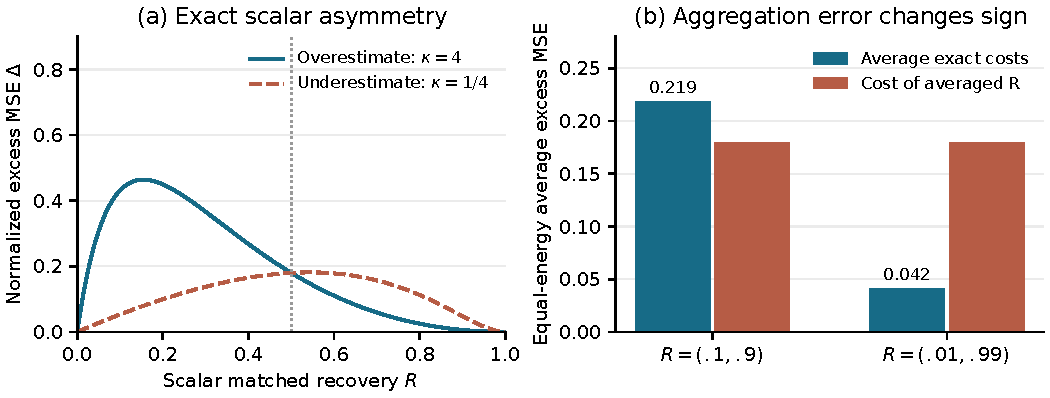
\includegraphics[width=.95\textwidth]{figures/scalar-cost.pdf}
\caption{Classical scalar cost and aggregation limits. Reciprocal mismatches cross at $R=.5$ under fixed effective noise. Equal-energy modes with the same mean $R=.5$ and $\kappa=4$ can give aggregation errors of either sign. These calculations do not identify a nonlinear network's effective prior.}\label{fig:cost}
\end{figure*}

\paragraph{Reference labels, not natural boundaries.} Historical protocols partition reference recovery at $.1$ and $.8$: A denotes high reference recovery, B intermediate and C low. These fixed labels permit the original test criteria to be audited. Their sensitivity has not been established, so we do not recommend them as deployment thresholds. With a fixed finite $\kappa$, the scalar excess vanishes as $R\to0$ or $1$, but the low-$R$ limit is not uniform over large mismatch factors. No reference label identifies the causal bottleneck of a trained decoder.

\paragraph{Band approximation.} A diagnostic sum
\begin{equation}\label{eq:crit}
C(Q)=\sum_b E_b\,\Delta\big(R_b,\kappa_b(Q)\big)
\end{equation}
substitutes measured band energies, reference recoveries and ratios of spectrum integrals. It is not the exact risk for a general operator. Its ranking accuracy and winner selection are distinct tests (\S\ref{sec:boundary}). Averaging $R$ and $\kappa$ before the nonlinear formula can either over- or under-estimate the true sum. For a fixed linear estimator the matrix expression in \S\ref{sec:setup} instead evaluates the specified covariance law directly.

\paragraph{No network mechanism follows.} A trained ASISR decoder is not a fixed Wiener estimator with known $\kappa$. Its measured $\Rnet$ is a truth-dependent outcome. Values near zero or one do not force a small readout-ablation loss: removing a component may improve a poorly recovered band or damage a perfectly recovered one. The loss ordering and scale-marginalisation tests below therefore require empirical evidence independent of the scalar identity.
